%!TEX root = forallxsol.tex
%\part{Interpretations}
%\label{ch.semantics}
%\addtocontents{toc}{\protect\mbox{}\protect\hrulefill\par}

\setcounter{chapter}{20}
\chapter{Truth in FOL}\setcounter{ProbPart}{0}
\problempart
\label{pr.TorF1}
Consider the following interpretation:
	\begin{ebullet}
		\item The domain comprises only Corwin and Benedict
		\item `$Ax$' is to be true of both Corwin and Benedict
		\item `$Bx$' is to be true of Benedict only
		\item `$Nx$' is to be true of no one
		\item `$c$' is to refer to Corwin
	\end{ebullet}
Determine whether each of the following sentences is true or false in that interpretation:
\begin{earg}
\item $Bc$ \hfill \myanswer{False}
\item $Ac \eiff \enot Nc$ \hfill \myanswer{True}
\item $Nc \eif (Ac \eor Bc)$ \hfill \myanswer{True}
\item $\forall x Ax$ \hfill \myanswer{True}
\item $\forall x \enot Bx$ \hfill \myanswer{False}
\item $\exists x(Ax \eand Bx)$ \hfill \myanswer{True}
\item $\exists x(Ax \eif Nx)$ \hfill \myanswer{False}
\item $\forall x(Nx \eor \enot Nx)$ \hfill \myanswer{True}
\item $\exists x Bx \eif \forall x Ax$ \hfill \myanswer{True}
\end{earg}

\problempart
\label{pr.TorF3}
Consider the following interpretation:	
	\begin{ebullet}
		\item The domain comprises only Lemmy, Courtney and Eddy
		\item `$Gx$' is to be true of Lemmy, Courtney and Eddy.
		\item `$Hx$' is to be true of and only of Courtney
		\item `$Mx$' is to be true of and only of Lemmy and Eddy
		\item `$c$' is to refer to Courtney
		\item `$e$' is to refer to Eddy
	\end{ebullet}
Determine whether each of the following sentences is true or false in that interpretation:
\begin{earg}
\item $Hc$ \hfill \myanswer{True}
\item $He$\hfill \myanswer{False}
\item $Mc \eor Me$ \hfill \myanswer{True}
\item $Gc \eor \enot Gc$ \hfill \myanswer{True}
\item $Mc \eif Gc$ \hfill \myanswer{True}
\item $\exists x Hx$ \hfill \myanswer{True}
\item $\forall x Hx$ \hfill \myanswer{False}
\item $\exists x \enot Mx$ \hfill \myanswer{True}
\item $\exists x(Hx \eand Gx)$ \hfill \myanswer{True}
\item $\exists x(Mx \eand Gx)$ \hfill \myanswer{True}
\item $\forall x(Hx \eor Mx)$ \hfill \myanswer{True}
\item $\exists x Hx \eand \exists x Mx$ \hfill \myanswer{True}
\item $\forall x(Hx \eiff \enot Mx)$ \hfill \myanswer{True}
\item $\exists x Gx \eand \exists x \enot Gx$ \hfill \myanswer{False}
\item $\forall x\exists y(Gx \eand Hy)$ \hfill \myanswer{True}
\end{earg}

\problempart
\label{pr.TorF3}
Following the diagram conventions introduced at the end of \S23, consider the following interpretation:	
\begin{center}
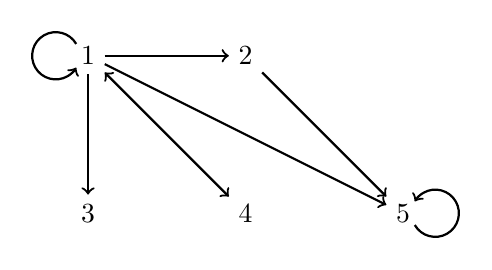
\begin{tikzpicture}
\node (atom1) at (0,2) {1};
\node (atom2) at (2,2) {2};
\node (atom4) at (0,0) {3};
\node (atom5) at (2,0) {4};
\node (atom6) at (4,0) {5};
\draw[->, thick] (atom1)+(-0.15,0.15) arc (-330:-30:.3); 
\draw[->, thick] (atom6)+(0.15,-0.15) arc (-150:150:.3); 
\draw[->, thick] (atom1) -- (atom2);
\draw[->, thick] (atom1) -- (atom4);
\draw[<->, thick] (atom1) -- (atom5);
\draw[->, thick] (atom1) -- (atom6);
\draw[->, thick] (atom2) -- (atom6);
\end{tikzpicture}
\end{center}
Determine whether each of the following sentences is true or false in that interpretation:
\begin{earg}
\item $\exists x Rxx$ \hfill \myanswer{True}
\item $\forall x Rxx$ \hfill \myanswer{False}
\item $\exists x \forall y Rxy$ \hfill \myanswer{True}
\item $\exists x \forall y Ryx$ \hfill \myanswer{False}
\item $\forall x \forall y \forall z ((Rxy \eand Ryz) \eif Rxz)$ \hfill \myanswer{False}
\item $\forall x \forall y \forall z ((Rxy \eand Rxz) \eif Ryz)$ \hfill \myanswer{False}
\item $\exists x \forall y \enot Rxy$ \hfill \myanswer{True}
\item $\forall x(\exists y Rxy \eif \exists y Ryx)$ \hfill \myanswer{True}
\item $\exists x \exists y (\enot x = y \eand Rxy \eand Ryx)$ \hfill \myanswer{True}
\item $\exists x \forall y(Rxy \eiff x = y)$ \hfill \myanswer{True}
\item $\exists x \forall y(Ryx \eiff x = y)$ \hfill \myanswer{False}
\item $\exists x \exists y(\enot x = y \eand Rxy \eand \forall z(Rzx \eiff y = z))$ \hfill \myanswer{True}
\end{earg}